\chapter{Kết quả thực nghiệm và đánh giá}
\label{chap:chap5}
\section{Kết quả thực nghiệm}
\begin{figure}[h]
    \centering
    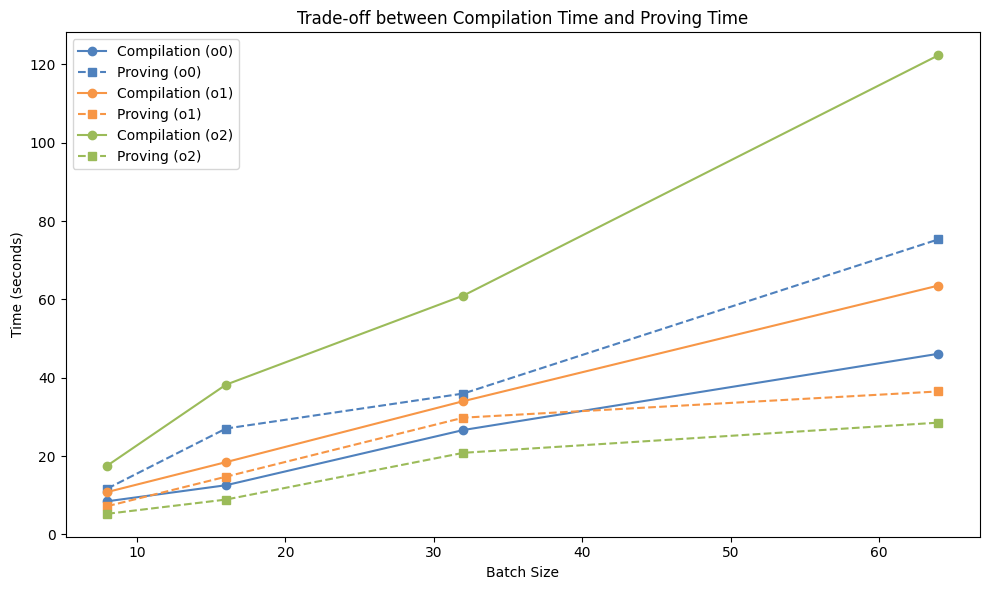
\includegraphics[width=\textwidth]{imgs/compilation_proving_time.png}
    \caption{So sánh thời gian biên dịch mạch và thời gian sinh chứng minh qua các mức tối ưu hóa khác nhau (--O0, --O1, --O2)}
    \label{fig:chapter5-compilation_proving_time}
\end{figure}

Từ Hình \ref{fig:chapter5-compilation_proving_time}, nghiên cứu nhận thấy một sự đánh đổi đáng kể khi áp dụng mức tối ưu hóa cao nhất trong quá trình biên dịch mạch. Cụ thể, thời gian biên dịch cho --O2 gần gấp đôi so với --O1 (165\% ở lô 64 giao dịch). Điều này nhấn mạnh rằng các nhà phát triển phải cân nhắc kỹ lưỡng khi chọn các cờ khác nhau cho các mục tiêu khác nhau trong quá trình phát triển các ứng dụng ZK.

\begin{figure}[H]
    \centering
    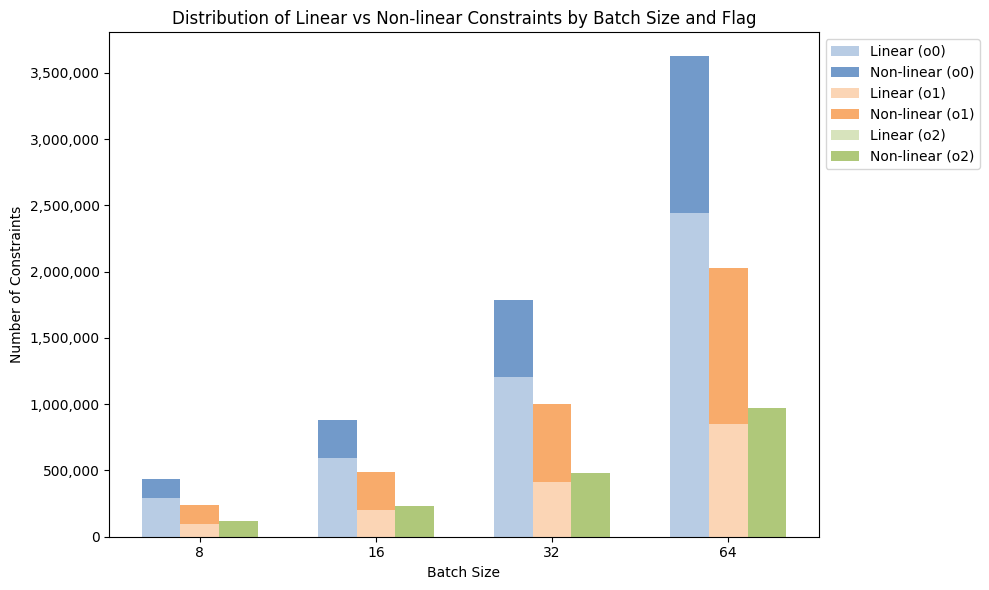
\includegraphics[width=\textwidth]{imgs/constraint_batchsize.png}
    \caption{Phân phối các ràng buộc tuyến tính và phi tuyến theo kích thước lô và cờ tối ưu hóa trình biên dịch.}
    \label{fig:chapter5-constraint_distribution}
\end{figure}

Hình \ref{fig:chapter5-constraint_distribution} cho thấy rằng cả --O1 và --O2 đều tối ưu hóa tốt cho các mạch xác minh theo lô. Việc giảm số lượng ràng buộc tuyến tính thông qua việc sử dụng các cờ tối ưu hóa khác nhau sẽ đóng góp trực tiếp vào hiệu quả của quá trình tạo bằng chứng.


\begin{table}[H]
    \centering
    \caption{Thời gian biên dịch và tạo bằng chứng trung bình cho mỗi tổ hợp kích thước lô và mức tối ưu hóa trình biên dịch.}
    \begin{tabular}{|c|c|c|c|}
        \hline
        \textbf{Kích Thước Lô} & \textbf{Cờ} & \textbf{Thời Gian Biên Dịch (s)} & \textbf{Thời Gian Tạo Bằng Chứng (s)} \\
        \hline
        8   & o0 & 8.458  & 11.696 \\
        8   & o1 & 10.818 & 7.204  \\
        8   & o2 & 17.557 & 5.264  \\
        \hline
        16  & o0 & 12.559 & 27.029 \\
        16  & o1 & 18.455 & 14.735 \\
        16  & o2 & 38.230 & 8.896  \\
        \hline
        32  & o0 & 26.661 & 35.975 \\
        32  & o1 & 34.030 & 29.811 \\
        32  & o2 & 60.991 & 20.838 \\
        \hline
        64  & o0 & 46.124 & 75.341 \\
        64  & o1 & 63.540 & 36.508 \\
        64  & o2 & 122.341 & 28.542 \\
        \hline
    \end{tabular}
    \label{tab:average_performance}
\end{table}

Bảng \ref{tab:average_performance} tóm tắt các chỉ số hiệu suất trung bình cho thời gian biên dịch và thời gian tạo bằng chứng qua các cấu hình khác nhau. Dữ liệu chỉ ra một cách rõ ràng rằng, trong khi --O2 giảm đáng kể số lượng ràng buộc, nó cũng kéo theo thời gian biên dịch cao hơn, nhấn mạnh các sự đánh đổi liên quan đến các chiến lược tối ưu hóa.

\section{Thảo Luận}

    \subsection{Câu hỏi nghiên cứu}
    
    Để làm rõ định hướng khi thực hiện thực nghiệm và phân tích, nghiên cứu này đặt ra hai câu hỏi nghiên cứu sau:
    \begin{itemize}
        \item Các mức tôi ưu hoá ràng buộc đã ảnh hưởng như thế nào đến các mạch ZK phức tạp như mạch xác minh lô giao dịch cho ZK-Rollup?
        % \item Làm thế nào để sử dụng được các mức tối ưu hoá của Circom trong thực tế một cách hiệu quả và nâng cao được hiệu suất của quá trình xây dựng và triển khai ZK-Rollup cũng như các ứng dụng ZK phức tạp khác.
        \item Phương pháp đề xuất \textbf{ZCLS} có góp phần đem lại cải thiện về hiệu suất cho nhà phát triển khi sử dụng các cờ tối ưu hoá của Circom trong quá trình phát triển mạch ZK không? 
        
        \item Khả năng mở rộng và thích ứng của \textbf{ZCLS} với các hệ thống thực tế như thế nào?
    \end{itemize}
    
    \subsection{Phân tích sự ảnh hưởng của các mức tối ưu hoá ràng buộc đối với các độ đo đã ghi nhận}

    Kết quả của các thí nghiệm của nghiên cứu làm nổi bật mối quan hệ phức tạp giữa tối ưu hóa ràng buộc và hiệu suất sinh chứng minh. Đặc biệt, việc sử dụng --O2 có tác động đáng kể đến thiết kế mạch. Bằng cách loại bỏ gần như tất cả các ràng buộc tuyến tính, như được chỉ ra bởi dữ liệu cho thấy các ràng buộc tuyến tính đã giảm xuống bằng không, --O2 tinh giản mạch R1CS, cho phép nó tập trung chủ yếu vào các ràng buộc phi tuyến còn lại. Mặc dù --O2 không giảm đáng kể số lượng ràng buộc phi tuyến, như bảng \ref{tab:average_performance} đã trình bày, số lượng ràng buộc phi tuyến chỉ giảm khoảng 18\% ở kích thước lô 64 so với --O0; nhưng --O2 đã thể hiện hiệu quả trong việc loại bỏ các ràng buộc tuyến tính, vốn không làm thay đổi cấu trúc logic của mạch Groth16. Sự tối ưu hóa này cho phép người chứng minh tập trung vào các ràng buộc phi tuyến, điều này rất quan trọng để duy trì tính toàn vẹn của quá trình sinh chứng minh.

    Bên cạnh đó, các kết quả thực nghiệm của nghiên cứu cho thấy phí gas cho việc xác minh vẫn ổn định qua các kích thước lô và số lượng ràng buộc khác nhau. Sự ổn định này có thể được giải thích bởi cho kiến trúc của Groth16, trong đó số lượng các phần tử trong bằng chứng cần được xác minh là cố định, bao gồm ba phần tử trên một đường cong elliptic \cite{groth2016size}. Ngoài ra, các đầu vào công khai, chẳng hạn như gốc (root) giao dịch, tương đối nhỏ và không ảnh hưởng đáng kể đến tổng chi phí gas.

    Tương tự, kích thước chứng minh rất ổn định nhờ vào cấu trúc cố định của nó, chỉ bao gồm ba phần tử trên đường cong elliptic. Đặc điểm này nhấn mạnh rằng trong khi tổng số lượng ràng buộc có thể thay đổi, kích thước chứng minh không dao động đáng kể với những thay đổi này.

    Trong bối cảnh ZK-Rollup và các giao dịch ERC-20, các hoạt động mật mã tiêu chuẩn như xác minh chữ ký và hàm băm tạo sẽ ra một số lượng lớn các ràng buộc phi tuyến. Thêm vào đó, các hoạt động logic trừu tượng hơn, chẳng hạn như quản lý và xác minh các chứng minh Merkle, cũng sử dụng các hoạt động mật mã này, dẫn đến việc sinh ra một khối lượng lớn các ràng buộc phi tuyến cho mạch ZK. Việc sử dụng --O2 hiệu quả trong việc cô đọng các ràng buộc chỉ còn những ràng buộc thiết yếu, từ đó tối ưu hóa quá trình sinh chứng minh.
    
    % \item \textbf{Phân tích về thời gian biên dịch của --O2}
    
    % Như đã đề cập trong Chương \ref{chap:chap3}, cờ tối ưu hóa --O2 của trình biên dịch Circom áp dụng các kỹ thuật nâng cao để giảm thiểu số lượng ràng buộc trong mạch R1CS, đặc biệt là sử dụng thuật toán khử Gauss dạng lười (Lazy Form of Gaussian Elimination). Mặc dù --O2 mang lại hiệu quả vượt trội trong việc giảm ràng buộc và tăng tốc độ tạo bằng chứng, quá trình biên dịch ở mức này lại tốn nhiều thời gian và tài nguyên tính toán hơn đáng kể so với -O0 và -O1. Điều này có thể được giải thích chi tiết hơn dựa trên cơ chế hoạt động nội bộ của trình biên dịch Circom và sự khác biệt trong các bước tiền xử lý so với -O1.

    \subsection{Kịch bản thử nghiệm kiểm tra ảnh hưởng của ZCLS với hiệu suất của việc phát triển ZK-Rollup}

    Các kịch bản này sử dụng dữ liệu thực nghiệm đã thu thập để mô phỏng hiệu quả của ZCLS trong
    các tình huống giả định thực tế:
    
\begin{enumerate}
    \item \textbf{Kịch bản 1: Giai đoạn gỡ lỗi chuyên sâu (Intensive Debugging Phase)}

    \begin{itemize}
    \item \textbf{Mô tả:} Một nhà phát triển đang trong giai đoạn gỡ lỗi một mạch ZK phức tạp với kích thước lô là 64. Trong một ngày làm việc, họ cần thực hiện 100 lần thay đổi nhỏ và biên dịch lại mạch để kiểm tra lỗi. Khối lượng tạo bằng chứng trong mỗi lần kiểm tra là rất thấp để kiểm tra tính chính xác của bằng chứng cơ bản.

    \item\textbf{Mục tiêu:} Giảm tối đa tổng thời gian chờ đợi biên dịch để duy trì chu kỳ phản hồi nhanh.

    \item\textbf{Phân tích theo ZCLS sử dụng dữ liệu thực nghiệm:}
    \begin{itemize}
    \item Trong trường hợp "Tần suất cập nhật mạch Rất Cao" và "Khối lượng tạo bằng chứng Rất Thấp", cờ --O0 được khuyến nghị.
    \item Thời gian biên dịch trung bình của --O0: 46.124 giây.
    \item Thời gian biên dịch trung bình của --O1: 63.540 giây.
    \item Thời gian biên dịch trung bình của --O2: 122.341 giây.
    \end{itemize}

    \item\textbf{Kết quả:}
    \begin{itemize}
    \item Sử dụng --O0: Tổng thời gian biên dịch = 100 lần * 46.124 giây/lần = 4612.4 giây (khoảng 76.87 phút).
    \item Sử dụng --O1: Tổng thời gian biên dịch = 100 lần * 63.540 giây/lần = 6354 giây (khoảng 105.9 phút).
    \item Sử dụng --O2: Tổng thời gian biên dịch = 100 lần * 122.341 giây/lần = 12234.1 giây (khoảng 203.9 phút).
    \end{itemize}

    \item\textbf{Lợi ích đem lại:} Trong kịch bản này, việc tuân thủ ZCLS và sử dụng --O0 giúp nhà phát triển tiết kiệm được khoảng 29 phút (giảm khoảng 27.4\% thời gian) so với --O1 và 127 phút (giảm khoảng 62.3\% thời gian) so với --O2 trong mỗi ngày gỡ lỗi. Điều này giúp duy trì năng suất cao và giảm sự gián đoạn trong quá trình làm việc.

\end{itemize}

\item \textbf{Kịch bản 2: Triển khai thực tế với khối lượng giao dịch lớn (Production Deployment with High Transaction Volume)}

\begin{itemize}
\item\textbf{Mô tả:} Một ZK-Rollup đã được triển khai và đang xử lý hàng chục nghìn giao dịch mỗi ngày. Mạch ZK đã ổn định và tần suất cập nhật mạch là rất thấp. Mục tiêu chính là tối thiểu hóa thời gian tạo bằng chứng để đạt được thông lượng cao và giảm chi phí vận hành.

\item\textbf{Mục tiêu:} Giảm tối đa thời gian tạo bằng chứng để tối đa hóa thông lượng và hiệu quả chi phí.

\item\textbf{Phân tích theo ZCLS với dữ liệu thực nghiệm:}
\begin{itemize}
    \item Trong trường hợp "Tần suất cập nhật mạch Thấp" và "Khối lượng tạo bằng chứng Cao", cờ --O2 được khuyến nghị.
    \item Thời gian tạo bằng chứng trung bình của --O0: 75.341 giây.
    \item Thời gian tạo bằng chứng trung bình của --O1: 36.508 giây.
    \item Thời gian tạo bằng chứng trung bình của --O2: 28.542 giây.
\end{itemize}

\item\textbf{Kết quả:}
\begin{itemize}
    \item Giả sử hệ thống cần tạo 1000 bằng chứng mỗi ngày.
    \item Sử dụng --O0: Tổng thời gian tạo bằng chứng = 1000 * 75.341 giây = 75341 giây (khoảng 20.9 giờ).
    \item Sử dụng --O1: Tổng thời gian tạo bằng chứng = 1000 * 36.508 giây = 36508 giây (khoảng 10.1 giờ).
    \item Sử dụng --O2: Tổng thời gian tạo bằng chứng = 1000 * 28.542 giây = 28542 giây (khoảng 7.9 giờ).
\end{itemize}

\item\textbf{Lợi ích đem lại:} Việc tuân thủ ZCLS và sử dụng --O2 giúp giảm đáng kể tổng thời gian tạo bằng chứng, từ đó tăng thông lượng giao dịch và cải thiện hiệu suất ZK-Rollup. So với --O0, --O2 giúp tiết kiệm khoảng 13 giờ thời gian tạo bằng chứng cho 1000 bằng chứng, và so với --O1 là 2.2 giờ. Điều này trực tiếp chuyển thành thông lượng cao hơn và khả năng mở rộng tốt hơn cho ZK-Rollup.
\end{itemize}

    \end{enumerate}
%     Các phát hiện cũng nhấn mạnh rằng thời gian biên dịch là một rào cản phát triển đáng kể cho các triển khai ZK-Rollup quy mô lớn. Mặc dù cần thiết phải sử dụng --O2 để đảm bảo sinh chứng minh hiệu quả, sự đánh đổi với thời gian biên dịch tăng lên có thể làm gián đoạn quy trình làm việc khi phát triển ứng dụng. Điều này cần một cách tiếp cận phát triển hai giai đoạn: trong các giai đoạn xây dựng và thử nghiệm, các nhà phát triển nên sử dụng --O1 làm mặc định để tối ưu hóa hiệu quả quy trình làm việc, trong khi chuyển sang --O2 cho sản xuất để tối đa hóa hiệu quả tạo bằng chứng.

%     Để hướng dẫn các nhà phát triển trong việc lựa chọn cờ tối ưu hóa, chúng tôi đề xuất một khung, như được trình bày trong Bảng \ref{tab:optimization_flag_selection} và Hình \ref{fig:chapter5-framework}, dựa trên tần suất cập nhật mạch và khối lượng chứng minh cần được sinh ra:

% \begin{itemize}
%     \item \textbf{Tần Suất Cập Nhật Mạch Cao:} Ưu tiên thời gian biên dịch nhanh để tăng tốc phát triển và giảm thời gian chờ cho các sửa đổi mạch.
%     \item \textbf{Tần Suất Cập Nhật Mạch Thấp:} Ưu tiên thời gian sinh chứng minh thấp, vì mạch sẽ được sử dụng để sinh nhiều chứng minh trong các hoạt động thực tế.
%     \item \textbf{Khối Lượng Sinh Chứng Minh Lớn:} Tối ưu hóa để giảm tổng thời gian sinh chứng minh.
%     \item \textbf{Khối Lượng Sinh Chứng Minh Nhỏ:} Chấp nhận thời gian chứng minh cao hơn để đổi lấy thời gian biên dịch nhanh hơn.
% \end{itemize}

% \begin{table}[h]
%     \centering
%     \caption{Các mức tối ưu hóa trình biên dịch Circom được khuyến nghị dựa trên giai đoạn phát triển, tần suất cập nhật mạch và khối lượng bằng chứng được tạo.}
%     \resizebox{\textwidth}{!}{%
%     \begin{tabular}{|l|l|l|l|}
%         \hline
%         \textbf{Giai Đoạn Phát Triển} & \textbf{Tần Suất Cập Nhật Mạch} & \textbf{Khối Lượng Tạo Bằng Chứng} & \textbf{Cờ Được Khuyến Nghị} \\
%         \hline
%         Phát Triển, Thử Nghiệm & Cao & Thấp & --O1 \\
%         Phát Triển, Thử Nghiệm & Cao & Cao & --O1 \\
%         Triển Khai Thực Tế & Thấp & Cao & --O2 \\
%         Triển Khai Thực Tế & Thấp & Thấp & --O2 \\
%         Trường Hợp Đặc Biệt (Gỡ Lỗi) & Rất Cao (Thường Xuyên) & Rất Thấp & --O0 \\
%         \hline
%     \end{tabular}
%     }
%     \label{tab:optimization_flag_selection}
% \end{table}

% \begin{figure}[h] % 'h' để đặt ảnh gần vị trí lệnh
%     \centering % Căn giữa ảnh
%     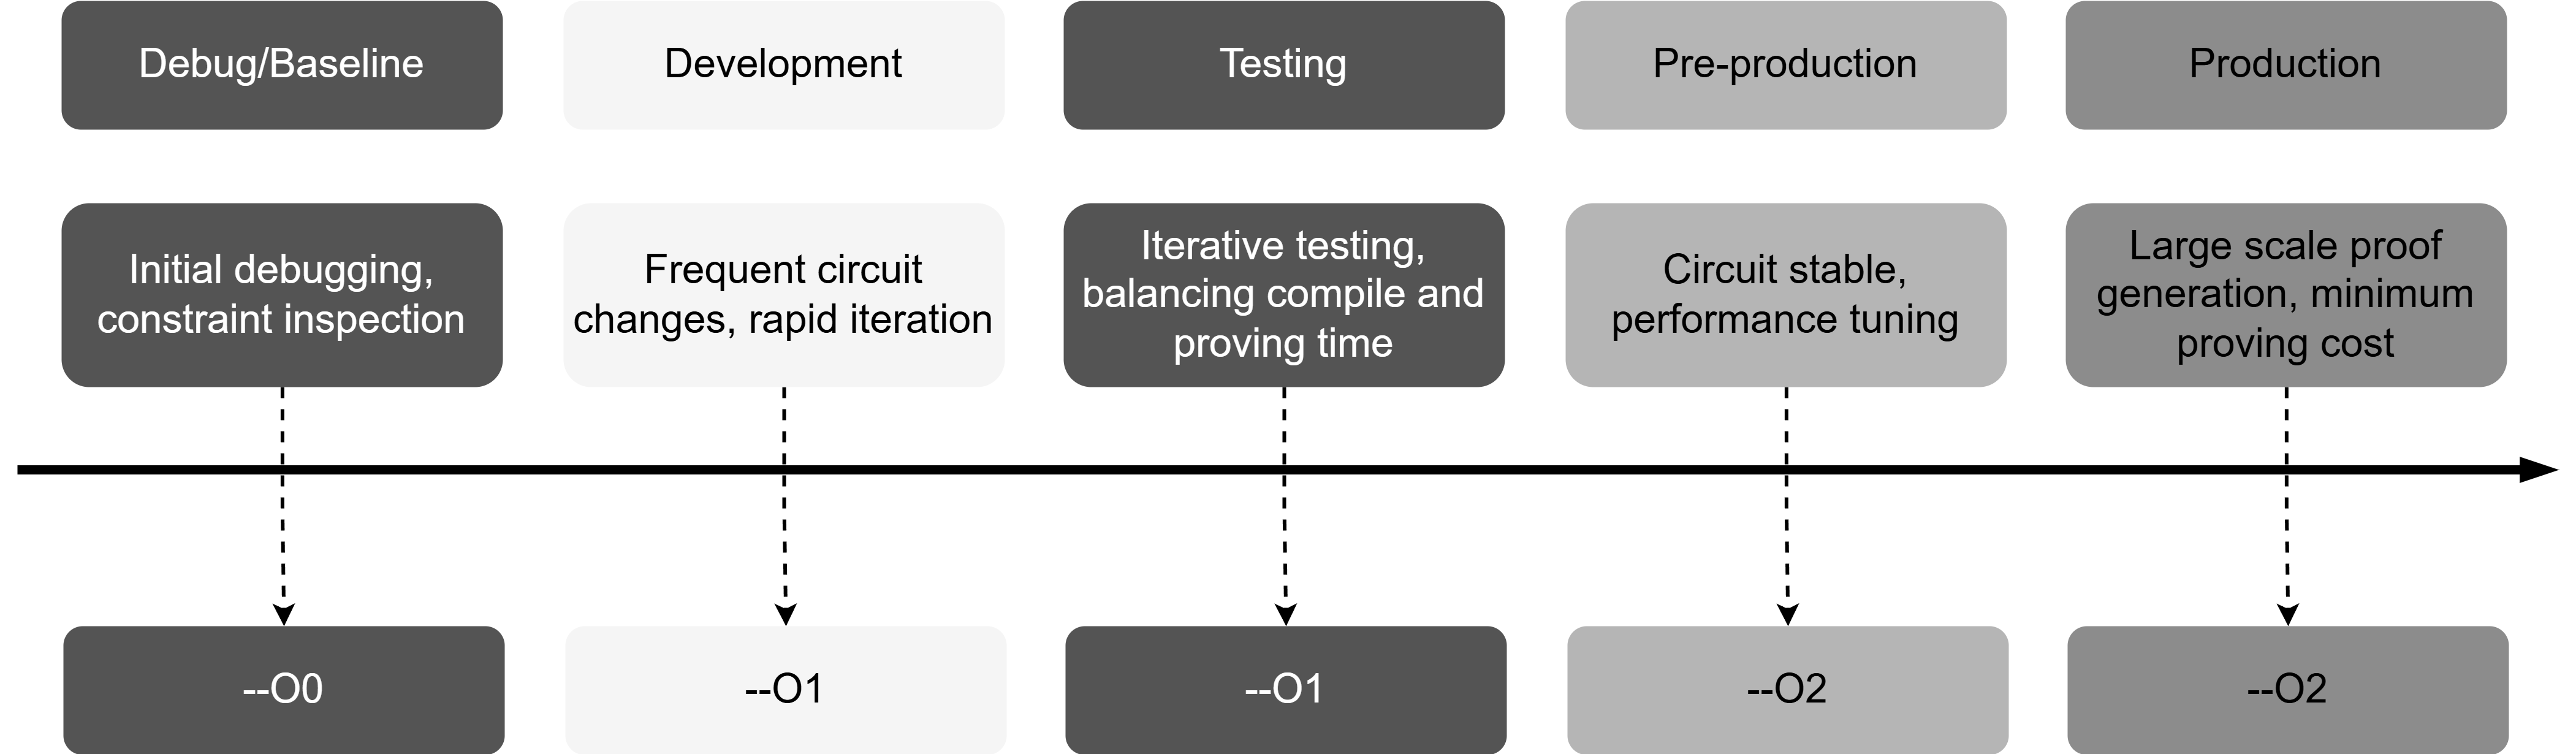
\includegraphics[width=\textwidth]{imgs/framework.png}
%     \caption{Khung chọn cờ tối ưu hóa trình biên dịch Circom dựa trên giai đoạn phát triển, tần suất cập nhật mạch và khối lượng tạo bằng chứng}
%     \label{fig:chapter5-framework}
% \end{figure}

    \subsection{Khả năng mở rộng và thích ứng của ZCLS với các hệ thống thực tế}

    Nghiên cứu này nhận thức rằng các thử nghiệm hiện tại được thực hiện với kích thước lô tối đa là 64. Trong thực tế, các hệ thống ZK-Rollup có thể xử lý các lô giao dịch lên đến vài nghìn hoặc thậm chí hàng chục nghìn, dẫn đến số lượng ràng buộc và thời gian biên dịch/tạo bằng chứng sẽ tăng lên đáng kể. Do đó, các giá trị được dùng trong phần giải thích khung cần được hiểu là dựa trên dữ liệu trong phạm vi thử nghiệm của nghiên cứu.

    Tuy nhiên, \textbf{nguyên lý cốt lõi và xu hướng} về sự đánh đổi giữa thời gian biên dịch và thời gian tạo bằng chứng giữa các cờ tối ưu hóa (--O0, --O1, --O2) vẫn sẽ được duy trì ngay cả ở quy mô lớn hơn. Cụ thể:

    \begin{itemize}
    \item --O0 sẽ là lựa chọn nhanh nhất về biên dịch nhưng chậm nhất về tạo bằng chứng.
    \item --O2 sẽ là lựa chọn chậm nhất về biên dịch nhưng nhanh nhất về tạo bằng chứng.
    \item --O1 sẽ cung cấp sự cân bằng hợp lý giữa hai yếu tố này.
    \end{itemize}

    % Tuy nhiên, nguyên lý cốt lõi và xu hướng về sự đánh đổi giữa thời gian biên dịch và thời gian tạo bằng chứng giữa các mức cờ tối ưu hóa (–O0, –O1, –O2) vẫn được duy trì ngay cả khi mở rộng quy mô. Cụ thể, cờ –O0 cho phép thời gian biên dịch nhanh nhất nhưng dẫn đến thời gian tạo bằng chứng chậm nhất. Ngược lại, cờ –O2 đòi hỏi thời gian biên dịch dài hơn song mang lại hiệu quả cao nhất trong việc rút ngắn thời gian tạo bằng chứng. Trong khi đó, cờ –O1 đóng vai trò trung gian, cung cấp sự cân bằng hợp lý giữa hai yếu tố trên.
    
    Khung này sẽ cung cấp một cách tiếp cận có cấu trúc giúp các nhà phát triển đưa ra quyết định thông minh về các cờ tối ưu hóa trong Circom, đảm bảo rằng chiến lược được chọn phù hợp với các yêu cầu cụ thể của giai đoạn phát triển ứng dụng.

    Bằng cách cung cấp dữ liệu thực nghiệm và một khung đề xuất để chọn các cờ tối ưu, nghiên cứu này mở rộng hơn các thảo luận lý thuyết về hiệu suất ZKP, cung cấp hướng dẫn thực tiễn cho việc phát triển các ứng dụng phi tập trung (DApps) và ứng dụng ZK trong các tình huống thực tế. Khung tối ưu hóa được đề xuất cho phép các nhà phát triển kiểm soát độ phức tạp của việc sinh ZKP, giảm thiểu thời gian thử nghiệm và sai sót, và tăng tốc độ triển khai ứng dụng.



